\documentclass{article}
% main document, called main.tex
\usepackage{tikz}
\usetikzlibrary{external}

\usetikzlibrary{positioning}
\usetikzlibrary{calc}
\usetikzlibrary{shapes.geometric, arrows, arrows.meta}
\usepackage{varwidth}% http://ctan.org/pkg/varwidth
\usetikzlibrary{shadows,trees, mindmap}
\usetikzlibrary{matrix}
\usetikzlibrary{fit}

\tikzexternalize % activate!
\begin{document}

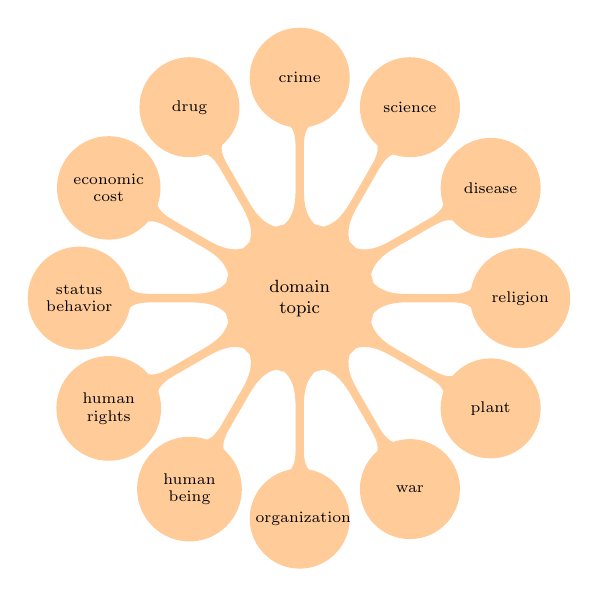
\begin{tikzpicture}

\path [small mindmap, grow cyclic, level 1/.append style={sibling angle=360/12},
root /.append style={font=\scriptsize},
every node/.append style={scale=0.8},
concept color=orange!40,
]
node [concept] {domain \\ topic}[clockwise from=0]
	child { node[concept] {religion}}
	child { node [concept]{plant}}
	child { node[concept] {war}}
	child { node[concept] {organization}}
	child { node[concept] {human being}}
	child { node[concept]  {human rights}}
  child {  node[concept] {status behavior}}
  child {  node[concept] {economic cost}}
  child {  node[concept] {drug}}
  child {  node[concept] {crime}}
  child {  node[concept] {science}}
  child {  node[concept] {disease}};
  child {  node[concept] {society effect}};
	
\end{tikzpicture}


\end{document}



